%-----appendices
\begin{appendices}
\noappendicestocpagenum
\addappheadtotoc
\pagebreak
\chapter{LHe Order Requirement Checklist}
%-----appendices
\label{appendix:checklist-for-cooldown}


\begin{tabular}{ l r c }
  Date: \underline{\hspace{4cm}} & Name: \underline{\hspace{4cm}}
\end{tabular}

\begin{minipage}{\textwidth}
\paragraph{LHe transfer}
\begin{checklist}
 \item \{$\Box$ 500TL, $\Box$ LTL\} pumped down
 \item delivery dewar Goddard fittings assembled and ready
 \item two helium cylinders by gas manifold (one is full)
 \item dewar pressurization line is ready
 \item number of additional He cylinders on hand: \blankprompt
 \item dewar scale and weight record form is ready
 \item LHe thumper or probe/readout are ready
 \item heat gun is plugged in and reaches dewar
 \item cryo safety equipment is ready for LHe transfer
 \item walkie talkies charged
 \item 100TL installed in 100LD; bayonet attached to WTL

\end{checklist}
\end{minipage}

\begin{minipage}{\textwidth}
\paragraph{Fridge}
\begin{checklist}
 \item target material installed: \blankprompt
 \item MC spacer/dam installed
 \item MC Si room temp: \blankprompt
 \item AVS-47 room temp: Ch 0: \blankprompt, Ch 1: \blankprompt , Ch 2: \blankprompt  
 \item leak check MC indium seal \blankprompt mbar l/s
 \item \het{} circ loop VRT: \blankprompt mbar/day
 \item leak check IVC indium seal: \blankprompt mbar l/s
 \item leak check OVC: \blankprompt mbar l/s
 \item align fridge with beamline
 \item flow impedance through fridge observed
 \item \hef{} Lakeshore sensors read to computer

\end{checklist}
\end{minipage}

\begin{minipage}{\textwidth}
\paragraph{Pump station area - \het}
\begin{checklist}
 \item leak detector available
 \item \lnn{} trap regenerated
 \item \lnn{} trap dewar filled
 \item mash cleaned
 \item T$_1$: \blankprompt mbar, T$_2$: \blankprompt mbar, T$_3$: \blankprompt mbar
 \item flow meter on \het{} gas rack powered on and recording
 \item mash cleaning system is set up for runtime cleaning
 \item all pump oil view ports half full
\end{checklist}
\end{minipage}

\begin{minipage}{\textwidth}
\paragraph{Pump station area - \hef}
\begin{checklist}
 \item \{$\Box$ sep, $\Box$ shield, $\Box$ evap\} flowmeters working
 \item sep/shield purged \blankprompt{} times; backfilled with He gas
 \item evap purged \blankprompt{} times; backfilled with He gas
 \item all pump oil view ports half full
 \item reading on 2000L \lnn{} tank: \blankprompt\%
\end{checklist}
\end{minipage}

\begin{minipage}{\textwidth}
\paragraph{Gamma Vault}
\begin{checklist}
 \item 100LD Goddard fittings assembled and installed on 100LD
 \item install exhaust tubing on 100LD and run over wall
 \item 100LD LHe level probe readout reading to computer
 \item OVC pressure: \blankprompt mbar
 \item IVC pressure: \blankprompt mbar
 \item fridge heating tapes installed
 \item heat gun is plugged in and reaches 100LD Goddards 
\end{checklist}
\end{minipage}

\begin{minipage}{\textwidth}
\paragraph{Polarizing magnet}
\begin{checklist}
\item Goddard fittings inspected/installed
\item \lnn{} and LHe readouts working
\item power suppy HP 6061A ready
\item control programmer AMI 420 ready
\item heat gun with extension cord set up on magnet
\item cryo safety equipment placed on magnet stand
\item magnet/detector carriage installed
\end{checklist}
\end{minipage}

\begin{minipage}{\textwidth}
\paragraph{Holding magnet}
\begin{checklist}
 \item resistance across holding magnet: \blankprompt $\Omega$
 \item power supply AMI PS 12100 ready
 \item control programmer AMI 420 ready
 \item energy absorber AMI 601 ready
 \item cable plugged into fridge
\end{checklist}
\end{minipage}

\begin{minipage}{\textwidth}
\paragraph{Microwaves}
\begin{checklist}
 \item EIO water is filled and flowing
 \item laptop webcam working
 \item microwaves tested with power meter: \blankprompt mW
 \item microwave frequency tested: \blankprompt GHz
 \item microwave guide connected to fridge
 \item thermistors and water flow readouts work and read to computer
\end{checklist}
\end{minipage}

\begin{minipage}{\textwidth}
\paragraph{NMR}
\begin{checklist}
 \item NMR water is running
 \item PDP running
 \item NMR is tuned
 \item $\lambda$/2 cable reconnected after swing
\end{checklist}
\end{minipage}

\chapter{SLPM Conversion}
\label{appendix:slpm-conversion}
Some Hifrost documents from CERN refer to flow rates of \hef{} and \het{} in millimoles per second.  The formula to convert this flow rate to SLPM is
\begin{equation}
 \textrm{[SLPM]}=\left(\frac{60\textrm{ s}}{\textrm{min}}\right)\left(\frac{x\textrm{ mol}}{\textrm{s}}\right)\left(\frac{4\textrm{ g}}{\textrm{mol}}\right)\left(\frac{1\textrm{ L}}{0.1785\textrm{ g}}\right)
\end{equation}
for \hef{} and 

\begin{equation}
 \textrm{[SLPM]}=\left(\frac{60\textrm{ s}}{\textrm{min}}\right)\left(\frac{x\textrm{ mol}}{\textrm{s}}\right)\left(\frac{3.01\textrm{ g}}{\textrm{mol}}\right)\left(\frac{1\textrm{ L}}{0.135\textrm{ g}}\right)
\end{equation}
for \het{}\cite{linde-helium-3-sheet}, where [SLPM] is the standard flow volume, $x$ is the flow rate in mol/s, $k$ is the Boltzmann constant and the definitions for STP are a temperature of 273.15 K and a pressure of 100 kPa.

Figure \ref{fig:slpm-conversion} shows some values of SLPM to mmol/s flow.

\begin{figure}
\begin{tabular}{|c|c|c|}
\hline
 SLPM& mmol/s (\het)& mmol/s (\hef)\\
\hline
5&3.74&3.71\\
\hline
10&7.48&7.44\\
\hline
15&11.21&11.16\\
\hline
20&14.95&14.86\\
\hline
25&18.69&18.60\\
\hline
30&22.42&22.31\\
\hline
40&29.90&29.75\\
\hline
50&37.38&37.19\\
\hline
60&44.85&44.63\\
\hline
80&59.80&59.50\\
\hline
100&74.75&74.38\\
\hline

\end{tabular}
\caption{Flow rate conversion between mmol/s to SLPM for helium.}
\label{fig:slpm-conversion}
\end{figure} 

\chapter{Transfer Line Drawings}
\label{appendix:tl-drawings}

\begin{figure}[!h]
 \centering
 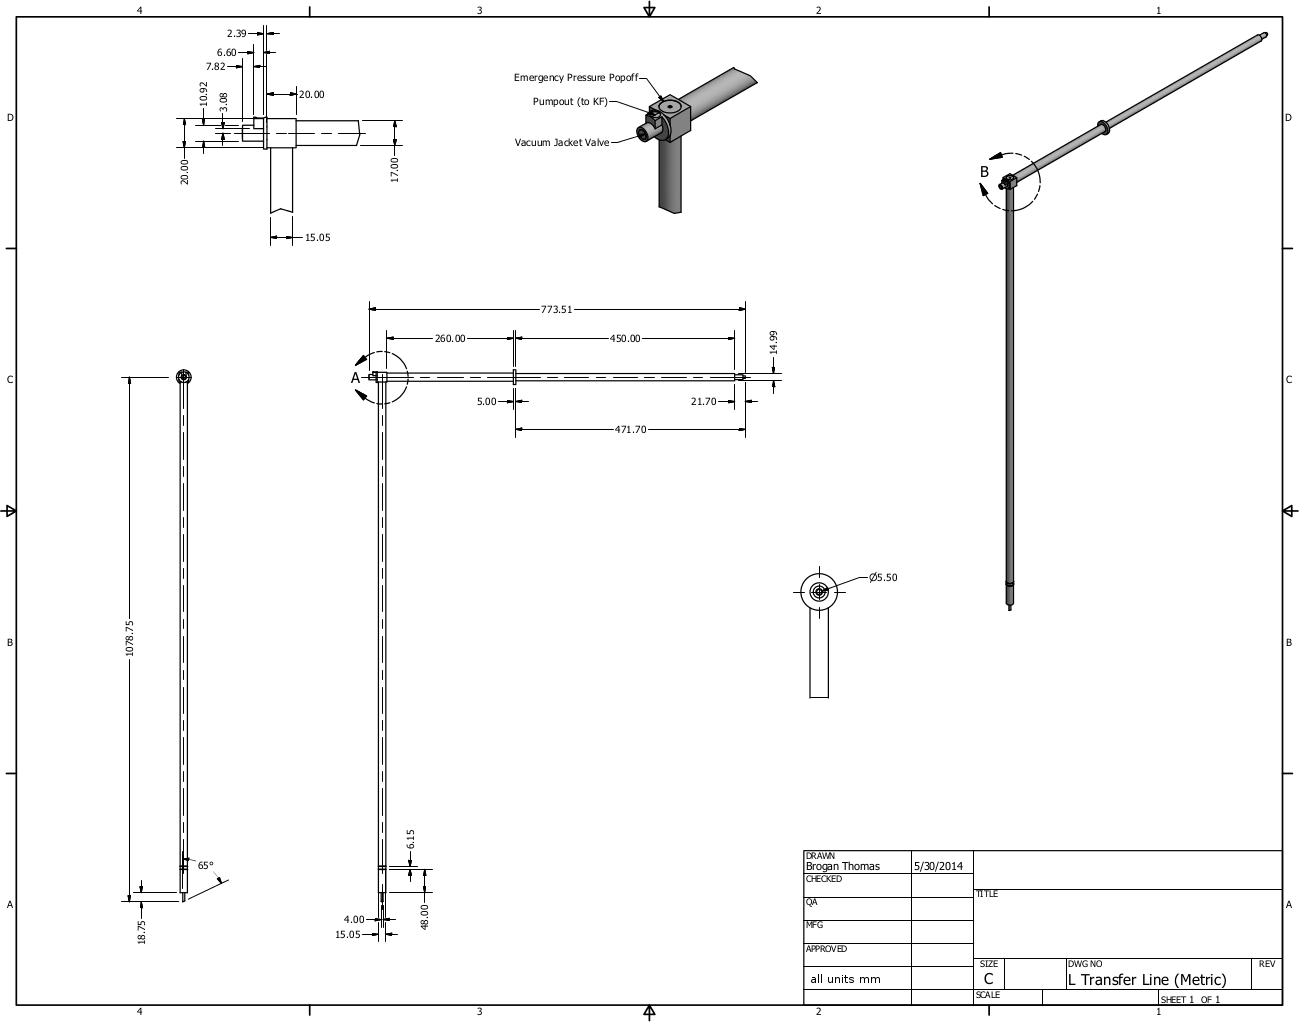
\includegraphics[width=\textwidth]{./img/LTL-drawing.png}
 \caption{Drawing of the LTL.}
 \label{fig:LTL-drawing}
\end{figure}

\begin{figure}[tbp!]
 \centering
 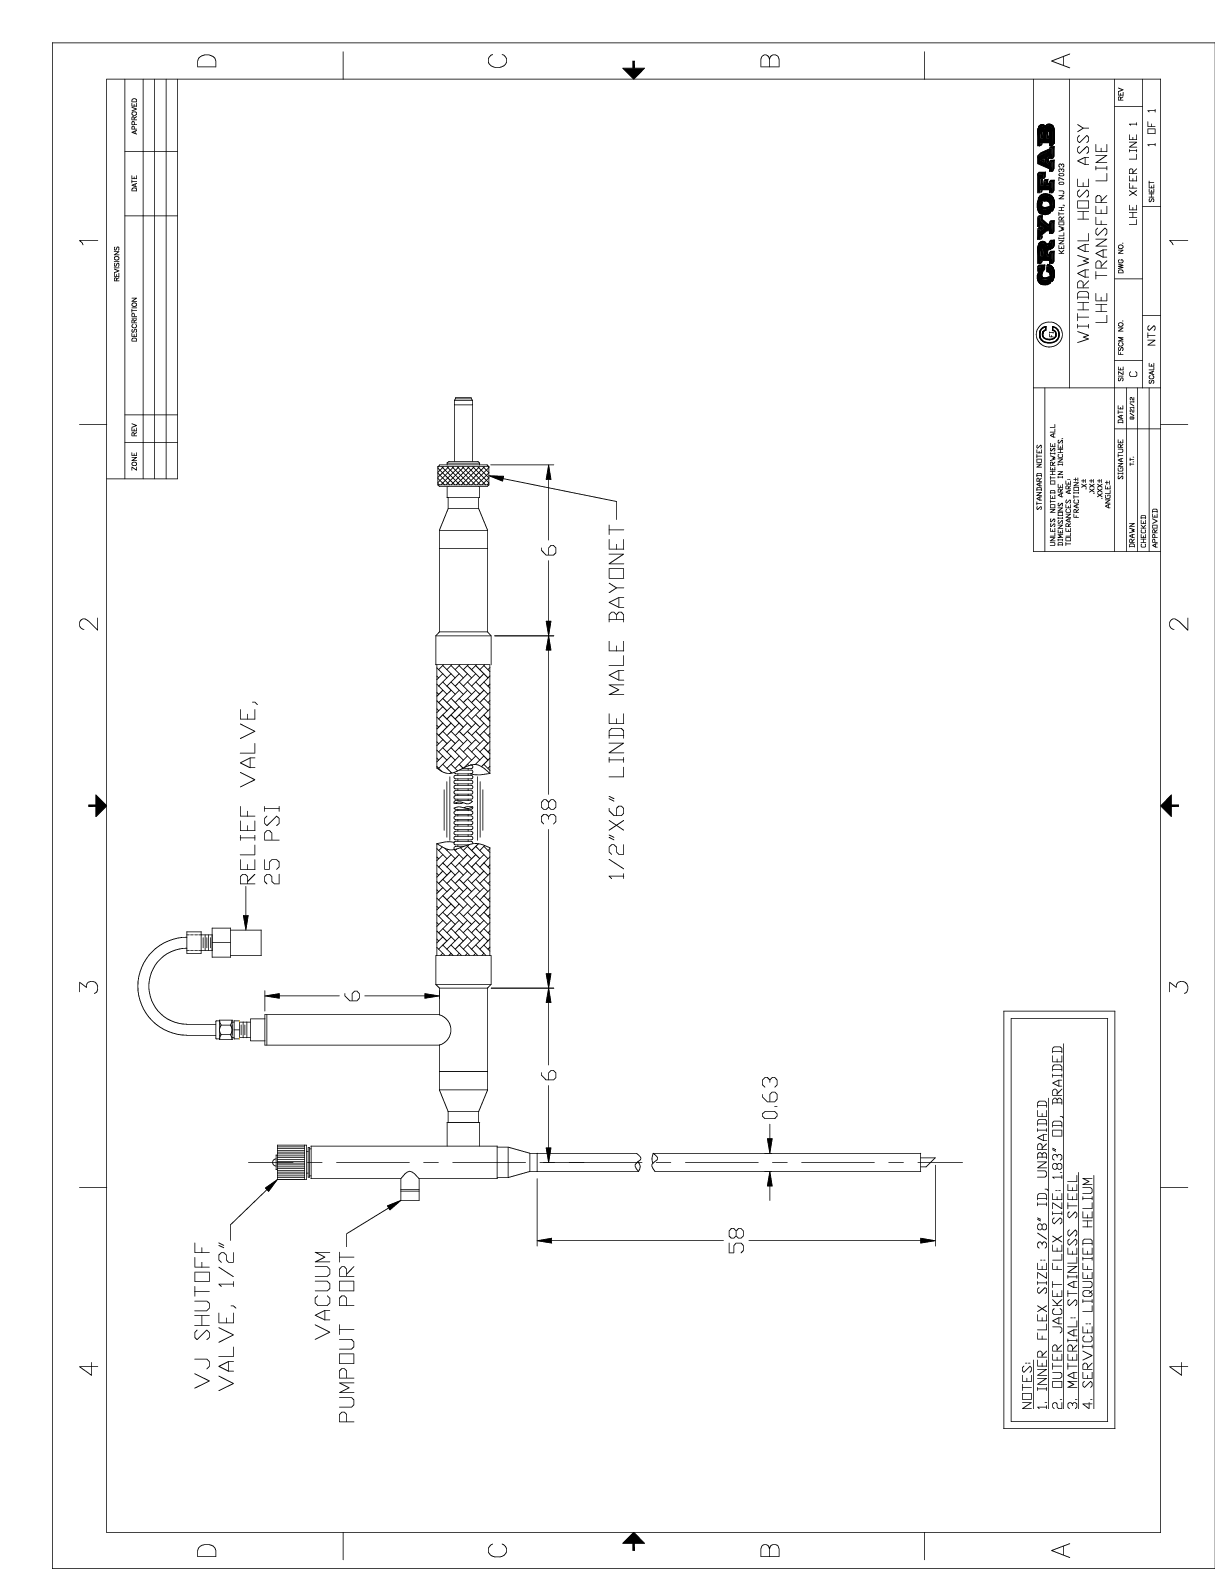
\includegraphics[width=\textwidth]{./img/500TL-drawing.png}
 \caption{Drawing of the 500TL.}
 \label{fig:500TL-drawing}
\end{figure}

\begin{figure}[tbp!]
 \centering
 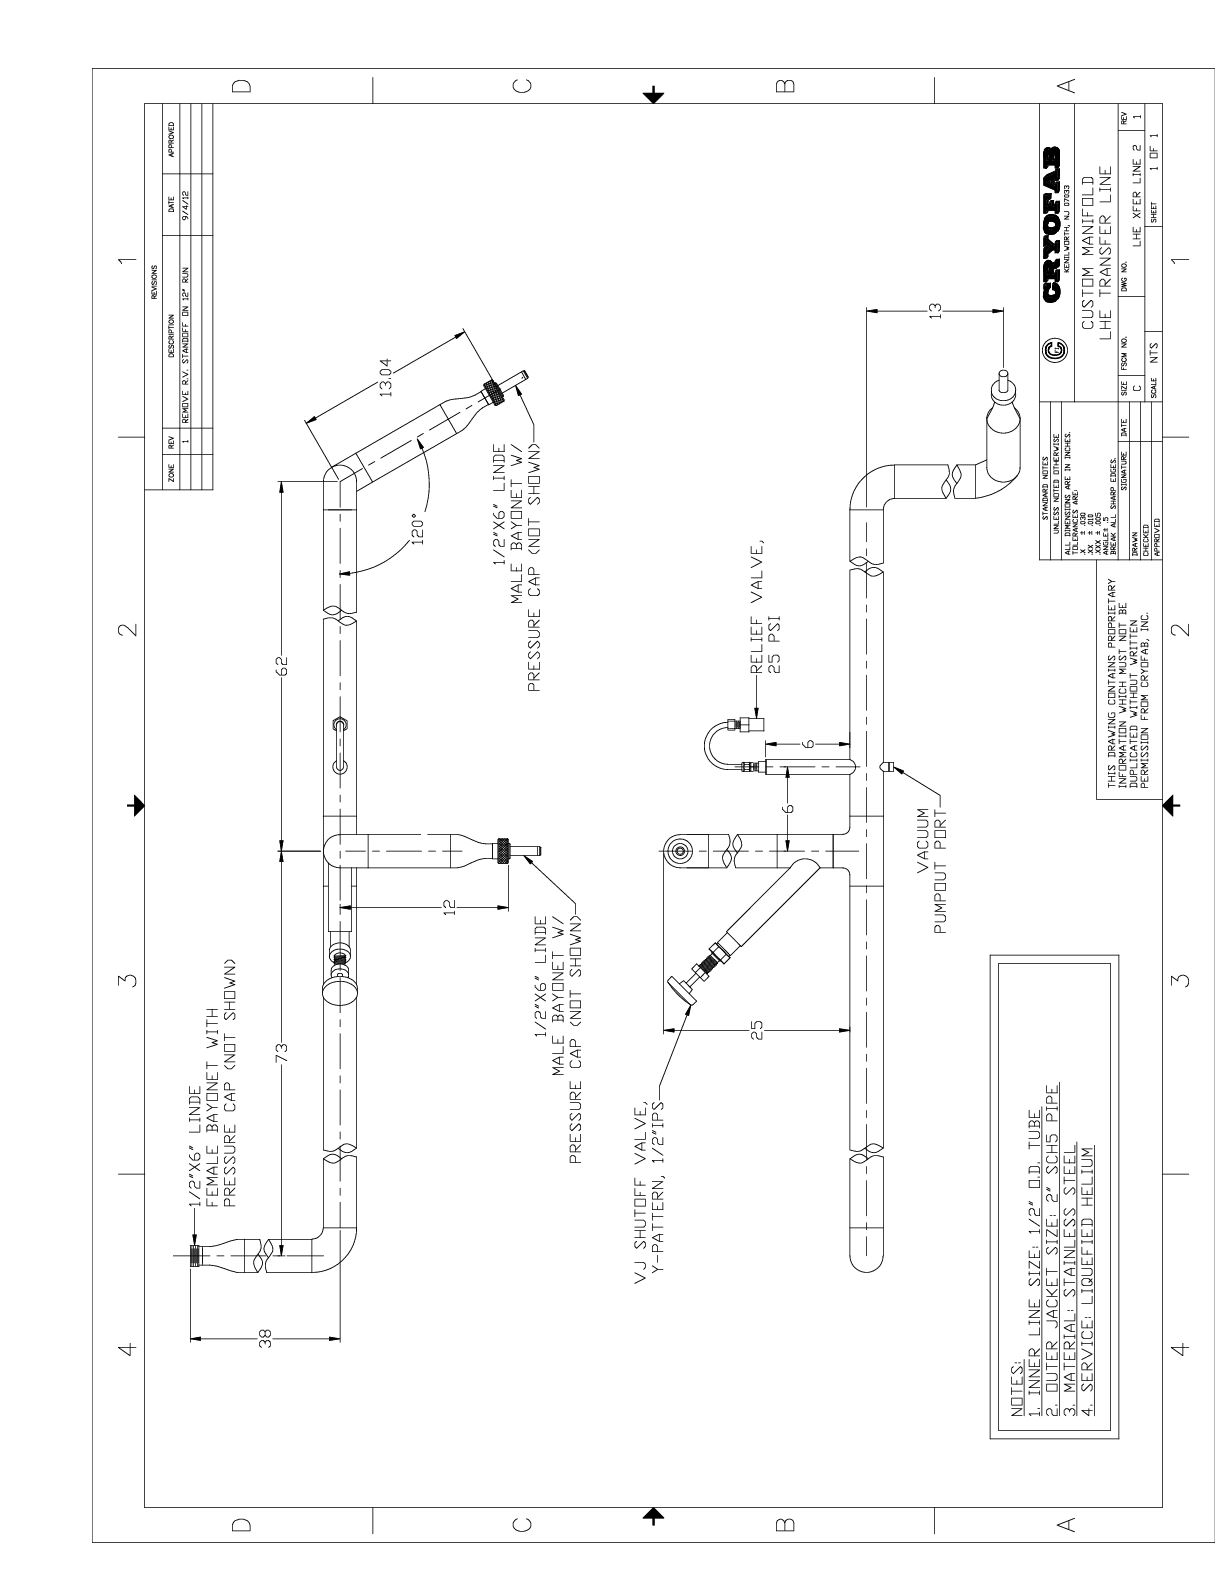
\includegraphics[width=\textwidth]{./img/WTL-drawing.png}
 \caption{Drawing of the WTL.}
 \label{fig:WTL-drawing}
\end{figure}

\begin{figure}[tbp!]
 \centering
 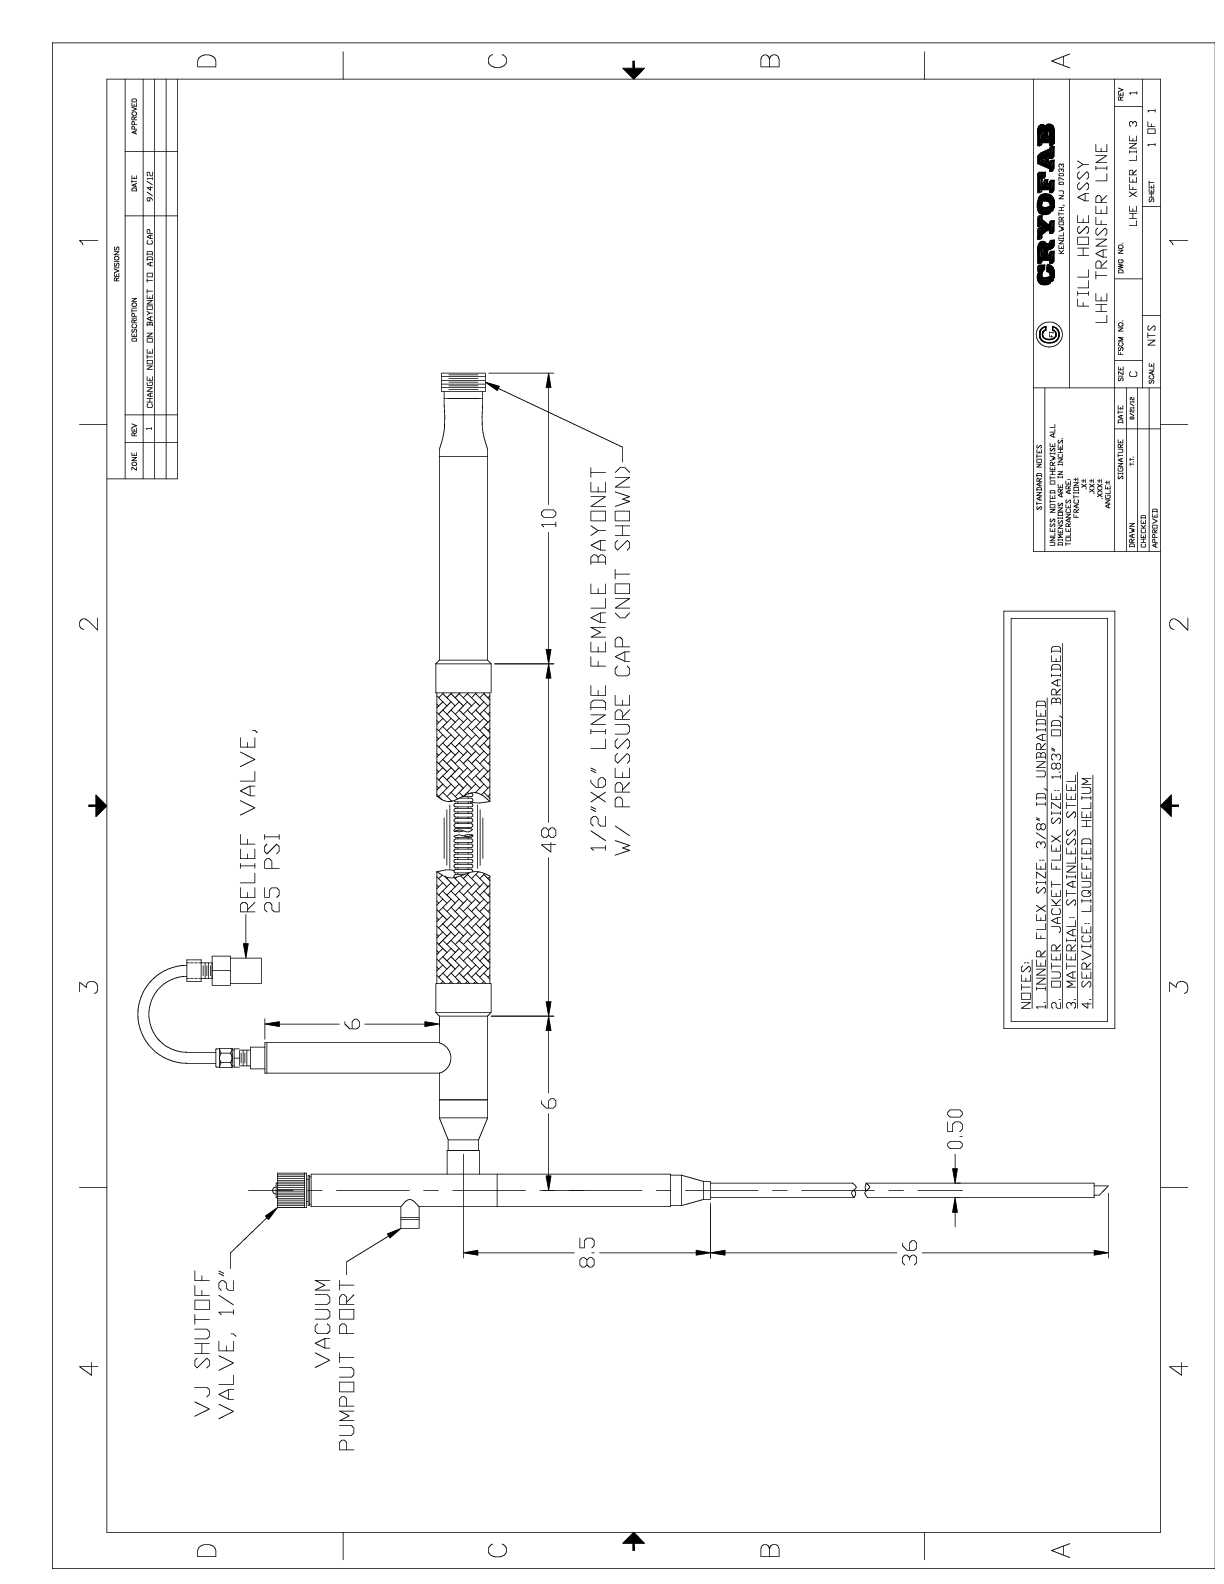
\includegraphics[width=\textwidth]{./img/MTL-drawing.png}
 \caption{Drawing of the MTL.}
 \label{fig:MTL-drawing}
\end{figure}

\begin{figure}[tbp!]
 \centering
 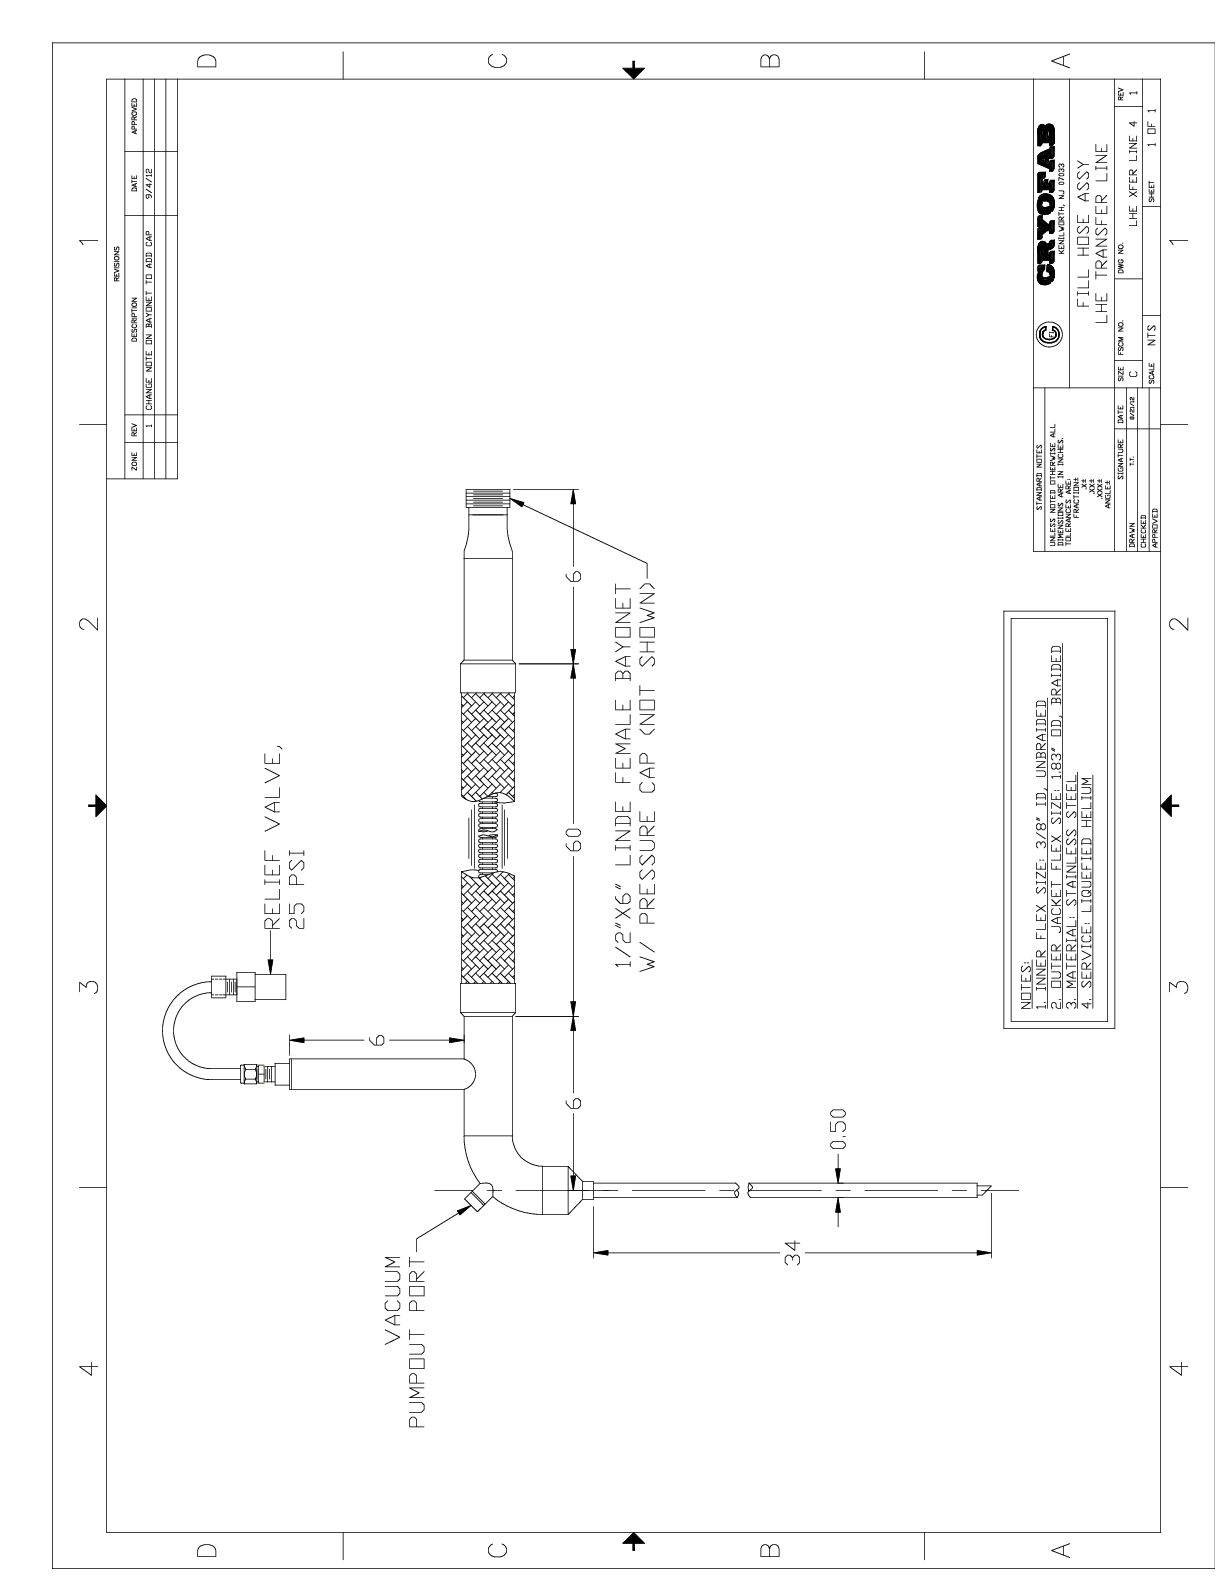
\includegraphics[width=\textwidth]{./img/100TL-drawing.png}
 \caption{Drawing of the 100TL.}
 \label{fig:100TL-drawing}
\end{figure}
\end{appendices}
